\documentclass[journal]{IEEEtran}
% \usepackage{times}
% \usepackage[small,compact]{titlesec}
% \usepackage[small,it]{caption}
% \usepackage{natbib}
% \usepackage{fullpage}
\usepackage{graphicx}
\usepackage[cmex10]{amsmath}
\interdisplaylinepenalty=2500

\title{Project Status Report: 3D Depth Reconstruction with Monocular Vision using Supervised Learning}
\author{Yiying Li}
\date{\today}

\begin{document}
\maketitle

\begin{abstract}
Generating depth from monocular vision (single image) is an interesting problem that humans solve fairly well. I replicated the work of Saxena et al. \cite{saxena2008} which takes a supervised learning approach. A training set is provided online containing various environments, such as indoor rooms, forests, building, etc, matched with their corresponding ground truth depth map generated by a 3D laser scanner system. Current research shows that depth estimation using a single image is difficult since local features of the image are insufficient, and global context is hard to define statistically. The algorithm implemented uses a hierarchical, Markov Random Field to model the image features to incorporate both local features as well as global context. Stereo vision can be augmented by this method to improve the areas in which stereo vision has difficulties, since monocular features and stereo geometric features are largely orthogonal. The current result of the reproduction is in progress, and the abstract will be updated to provide a short comparison in the final report.
\end{abstract}

\section{Introduction}
There is a lot of research on 3D reconstruction, and depth estimation using monocular vision. Most of them uses stereopsis vision \cite{scharstein2003}, or multiple images. Some also require multiple images, such as structure from motion \cite{Forsyth:2002:CVM:580035}. All of these focus on geometric differences that incorporate the use of triangulation. Humans can detect a lot of depth with one eye using monocular cues such as gradients, focus, coloring, and others. We also use these monocular cues along with stereo ones to figure out depth for ourselves. 

Depth estimation is still extremely difficult on a single still image, since there are a lot of ambiguity in local features. The algorithm must try and exploit some characteristic of the global structure of the image as well as try to use past experiences to augment the data. Depth extraction is extremely important to an overall bigger picture of scene understanding. 

\section{Visual Cues}
The visual cues that humans use are grouped into four categories by previous research \cite{loomis01, schwartz99}, monocular, stereo, motion parallax, and focus cues. We combine these to understand the 3D structure of the world, the model will try to combine most of the monocular cues and stereo cues to estimate depth.

Monocular cues are important to the estimation of depth. Texture gradients help capture the distribution of edge directions, which in turn indicate depth on a certain scale. A classic example is a tiled floor with parallel lines could appear to have tilted lines in an image. Haze is caused by light scattering which is another cue that certain objects are further away. There are many other cues such as occlusion, defocus, shading, shadows, etc. Most monocular cues are information of the global properties of the image, and thus can't be computed or inferred from local regions in the image, even if certain local information such as color could be an indicator. Overall properties of the entire image must be looked at to try and capture these monocular cues.

As a robot moves, close objects appear to move more than objects that are further away. This is an example of motion parallax cues. The ability to focus also causes certain object to be out of focus, this can be an indicator of depth as well. Stereo cues usually rely on some sort of geometric relation between the two cameras capturing the images. There is a downfall to stereo cues for object at distances extremely far away, it is hard to generate the relationship when you get to sub-pixel differences.

\section{Feature Extraction}
The image is divided into small rectangular patches, and a single depth value is estimated for each patch. There are two types of features used in this estimate, {\em absolute} depth features are used to estimate the depth at the specific depth and {\em relative} features which are used to estimate relative depth. Relative depth is the magnitude of the difference between the two patches. Absolute features map to local feature processing and relative features maps to continuity features for humans.

\begin{figure*}[!t]
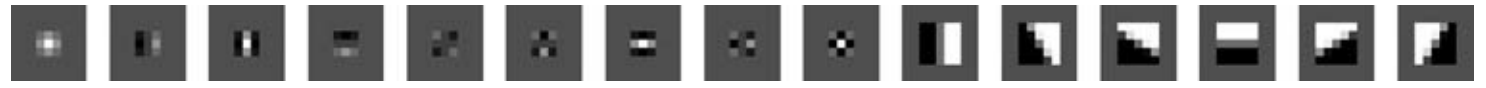
\includegraphics[width=\linewidth]{lawsmask.PNG}
\caption{The first 9 are laws' mask, and the rest are rotated edge detectors}
\label{fig:lawsmask}
\end{figure*}

\begin{figure*}[!t]
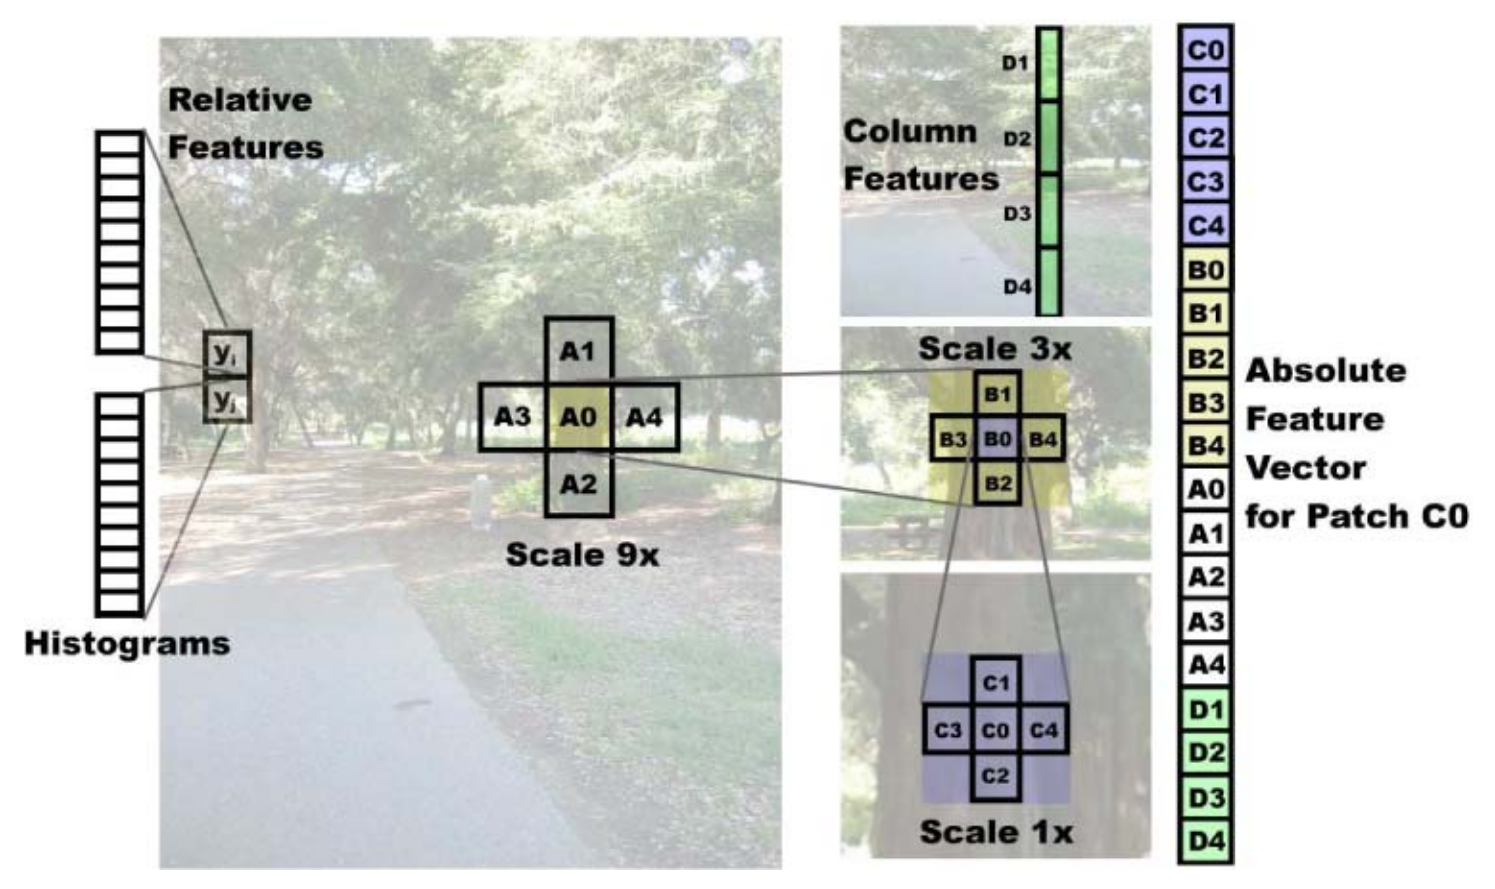
\includegraphics[width=\linewidth]{Features.PNG}
\caption{The absolute depth features vector is generated from the textual energies of a patch, its surrounding patches, the textual energies of the different scale patches centered on this patch, their surrounding patches, and the textual energies of vertical column patches. The relative features for each patch is a histogram of the different textual energies.}
\label{fig:featureimage}
\end{figure*}

Three types of local cues are captured: texture variation, texture gradients, and color. Texture variation is mostly contain in the intensity of the image, therefore we store the image in the YCbCr color format so we can isolate this channel. Laws' mask \cite{davies04, michels05} can be applied to this channel to compute texture energy (Figure \ref{fig:lawsmask}). Haze can be calculated by first applying the first Laws' mask, which is a local averaging filter, to each of the color channels. Texture gradients that are resistant to noise can be generated with size oriented edge filters. We split these features into absolute depth features and relative depth features. We calculate these textural energy on a patch of a certain size, we also have different scales for the patch size which can be see in Figure \ref{fig:featureimage}.

\subsection{Absolute Depth Features}
(need to add a image explaining how this works)

For each patch $i$ inside an image $I(x, y)$, where $x, y$ correspond to location of the patch. There are 17 outputs from the the filters (9 Laws' masks, 2 color, 6 texture gradients). Let these filter outputs be represented by $F_n, n = 1,..., 17$. Then the energy of each filter is calculated by
\begin{equation}
E_i(n, k) = \sum_{(x, y) \in patch(i)} |I * F_n|^k
\end{equation}
where $k \in \{1, 2\}$, this generates a feature vector of 34 elements.
This isn't enough as we need to incorporate more of the global properties. The author mentions that using more $k$ values doesn't affect the results at all. This is done by extract on multiple image resolutions. To capture these properties the features are computed from the neighboring four patches as well as the current patch. This is then repeated on 3 different scales (resolutions) and the neighbors on each scale. We also add a column vector that contains 4 column patches to account for vertical consistency. The column vector is size at the highest scale in order to capture the most potential consistency of the object. The full feature vector for this patch comes out to $19*34 = 646$ elements in the each feature vector for each patch.

\subsection{Relative Features}
A 10-bin histogram is calculated for each of the 17 $F_n$ filters, generating $170$ features for each patch at each scale. This is used to estimate the difference in depth between two different locations. This require less global information as if nearly by patches exhibit extremely similar properties then it is somewhat safe to consider them the same object. Relative depth features $y_{ijs}$ for two neighboring patches $i$ and $j$ on scale $s$ can be calculated from the difference of the histograms.

\section{Markov Random Field}
A Markov random field (MRF) is a set of random variables in a undirected graph where the variables have a Markov property. This provides a consistent and convenient way to model things that are context-dependent such as depth features. Nodes in $S$ are related to each other by a neighborhood system $N = \{N_i, i \in S\}$. This can be multi-dimensional and can also be characterized by a Gibbs distribution. There are many ways to train a MRF, the most popular way is to use maximum likelihood either over joint distribution or marginal likelihood.
The maximum joint likelihood can be used to train the Gaussian MRFs, however Laplacian MRFs are intractable using maximum joint likelihood as there is no close form to the partition function. Laplacian MRF's can be roughly estimated using the Gaussian approximation.

MRFs have a variety of uses in computer vision as many tasks can be posed as energy minimization problems on a rectangular grid of pixels. Some examples where MRFs have been used extensively is in problems such as denoising, finding the stereo disparity, reconstruct smooth surface given sparse measurements, and segmentation (aka foreground extraction). The key to using MRFs is that since there are a lot of local connections information from one point can propagate very far into another point on the graph. This is important to try and interpret local information on a global scale. We want to use this key feature for MRFs to try and propagate the local information of patches since even areas far away from each other may have can effect on the depth of those areas.
\section{Models}

\subsection{Gaussian Model}
The Gaussian Markov Random Field model is shown in Equation \ref{eq:gaussian_model}.
\setlength{\arraycolsep}{0.0em}
\begin{eqnarray}
\label{eq:gaussian_model}
P_G(d|X; \theta, \sigma) &{}={}& \frac{1}{Z_G}\exp\left(-\sum_{i=1}^{M}\frac{(d_i(1)-x_i^T\theta_r)^2}{2\sigma^2_{1r}} \vphantom{\sum_{j \in N_s(i)}}\right.\nonumber\\
&&- \left.\sum_{s=1}^3\sum_{i=1}^M\sum_{j \in N_s(i)} \frac{(d_i(s)-d_j(s))^2}{2\sigma_{2rs}^2}\right)
\end{eqnarray}
\setlength{\arraycolsep}{0.0em}

$M$ is the number of patches in the image at the lowest scale, $Z_G$ is the normalization constant, $x_i$ is the absolute depth feature vector for patch $i$, $\theta$ and $\sigma$ are the parameters of the model. These parameters are further parameterized by row $r$, since the images are assume to be taken from a horizontally mounted camera thus exhibiting similar properties. The depths are $d_i(s), s \in \{1, 2, 3\}$, the depth at higher scales are the average of the depths of the lower scales as indicated in Equation \ref{eq:higher_depth}
\begin{equation}
\label{eq:higher_depth}
d_i(s+1) = (1/5)\sum_{j \in N_s(i) \cup {i}} d_j(s)
\end{equation}
$N_s(i)$ are the neighbors of patch $i$ on scale $s$. The second summation term is a smoothing factor that depends on the variance parameters $\sigma_{2rs}^2$ to determine the amount of smoothing.

The variance term $\sigma_{2rs}^2$ is a linear function of patch $i$ and $j$'s relative depth features $y_{ijs}$. This is modeled as $\sigma_{2rs}^2 = u^T_{rs}|y_{ijs}|$, this helps with which neighboring patches are likely to have similar depth. The other variance term $\sigma^2_{1r} = v_x^T x_i$ is a linear function of the features, this gives a uncertainty measure as well as a dependency on features. The variables $u^T_{rs}$ and $v_x^T$ are fitted to their corresponding trained variances. Inference on this network is done with a MAP estimate (need to include the math for this). Log $P(d|X; \theta, \sigma)$ is quadratic, therefore the maximum is easily found.

\subsection{Laplacian Model}
The Laplacian model is show in Equation \ref{eq:laplace-model}.

\setlength{\arraycolsep}{0.0em}
\begin{eqnarray}
\label{eq:laplace-model}
P_L(d|X; \theta, \lambda) &{}={}& \frac{1}{Z_L}\exp\left(-\sum_{i=1}^{M}\frac{|d_i(1)-x_i^T\theta_r|}{\lambda_{1r}} \vphantom{\sum_{j \in N_s(i)}}\right.\nonumber\\
&&- \left.\sum_{s=1}^3\sum_{i=1}^M\sum_{j \in N_s(i)} \frac{|d_i(s)-d_j(s)|}{\lambda_{2rs}}\right)
\end{eqnarray}
\setlength{\arraycolsep}{0.0em}

The reason for this model is that the relative features in the form of a histogram are more Laplacian than Gaussian. This model also has much longer tails than Gaussian, therefore lending itself to be more robust to outliers which also producing sharp edges that the Gaussian model failed to do.

Maximum likelihood is intractable for a Laplacian model, since the partition depends on $\theta_r$. We can approximate by solving linear system of equations $X_r\theta_r \approx d_r$ to minimize $L_1$ norm errors ($min_{\theta_r}(||d_r-X_r\theta_r||_1$). The spread parameters are learned the same way as the Gaussian model except losing the exponents and adding absolute values. MAP inference is still tractable and convex, this can be solved using a linear program.

\section{Replication}
The replication was mostly done in MATLAB for its extensive image processing library, as well as its very optimized set of functions for linear regression as well as robust linear regression where we throw out outliars. As expected there were many difficulties in replication of this work. I will point them out before we get to the results because it is important to understand what couldn't be accomplished before looking at the results. I will break down the difficulties that I was able to overcome and the difficulties that I was not able to overcome. Many of these problems stemmed from insufficient information on the models as well as current hardware limitations. There are a few numbers that they don't provide and assumptions had to be made, the most important is the patch size of the lowest scale. I chose this to be a 8x8 patch as that reduced the 1704x2272 image to 213x284, which was as close as possible to the size of the depth map provided.

\subsection{Surmounted Difficulties}
The first task of feature generation was initially hard as they don't provide the values of the mask's they used for convolution to generate the features of the image. Fortunately Law's mask are a specific set of filters that are readily available in computer vision text book. The rotated edge filters, while the general form of an edge filter is simple, there is a problem of the scale and there is quite a bit of difference between the filter if Eq \ref{eq:filter1} and filter in Eq \ref{eq:filter2}. The scale also can vary the output slightly and potentially causing the regression to lean towards a certain value. I ended up just choosing the filter in Eq \ref{eq:filter1}, as it is more widely used in vision applications. Another problem that occurred with the edge filters is the rotation of the filters, if we just try to rotate these matrices by $30^{\circ}$ then there has to be some interpolation. Filters generally are integral numbers, therefore if use interpolation we have to fix the floating point numbers to integral numbers. When I did this it doesn't line up with what the author has presented in masks (Figure \ref{fig:lawsmask}). What I did was to go back and change all the values of the filters until they matched the output from the author, and I can only assume that I did this correctly as there is no way to know that the author and I chose the same form of visualization (however there isn't many different ways).
\begin{eqnarray}
\label{eq:filter1}
\begin{bmatrix}
	-2~&0~&-2 \\
	-2~&0~&-2 \\
	-2~&0~&-2 \\
\end{bmatrix}
\end{eqnarray}
\begin{eqnarray}
\label{eq:filter2}
\begin{bmatrix}
	-2~&1~&-2 \\
	-2~&1~&-2 \\
	-2~&1~&-2 \\
\end{bmatrix}
\end{eqnarray}

Once I started to do feature extraction I ran into many problems with the speed of the algorithm. Since we have to sum over all the pixels an extreme number of times as we have many patches and for each patch we also had to account for surrounding patches. With a very naive implementation this would have taken around 400 hours (16 days) for 400 images. I had to think of much more efficient way to calculate this, as the author doesn't tell you how to do this as I think this pretty far into implementation details. I still feel it is important to state how important and how much time it could have saved me if the author mentioned pre-computing certain things. With pre-computing the patches at only the lowest scale and a clever pre-computing on for the columns, I was able to achieve 100 seconds per image.

Running regression on the model for learning posed another interesting yet annoying and non-technical problem. The resulting features data from a single 1704x2272 images was around 280MB of data. If we wanted to train on 400 images, this would have required 112GB of RAM, which is infeasible. Instead we had to read from disk for every row that we wanted to run regression on. As expected loading a 280MB data from disk just to extract a row of features is extremely slow, so slow that it would have taken over a full year to do this for for each possible row (284). After much thought the rows of features are extracted independently and precomputed before training to reduce the loading time of each row feature set. This reduced the loading time substantially, however regression time can not be lowered from 400+s for each row.

\section{Replication Results}

\section{Conclusion}

\section*{Acknowledgment}
I would like to thank Chansoon Lee, and professor Benjamin Kuipers for helping me with the impossibly hard to understand parameters of the models described in this paper, preventing me from thinking that I was going crazy because nothing made sense.

\bibliographystyle{IEEEtran}
\bibliography{IEEEabrv, report}

\end{document}